\documentclass[a4paper,twoside,12pt]{article}
% Alternative Options:
%	Paper Size: a4paper / a5paper / b5paper / letterpaper / legalpaper / executivepaper
% Duplex: oneside / twoside
% Base Font Size: 10pt / 11pt / 12pt


%% Language %%%%%%%%%%%%%%%%%%%%%%%%%%%%%%%%%%%%%%%%%%%%%%%%%
\usepackage[english,french]{babel}
\usepackage[latin1]{inputenc}
\usepackage[T1]{fontenc}
\usepackage{ae}

\usepackage{lmodern} %Type1-font for non-english texts and characters

\usepackage[top=2.5cm, bottom=2cm, left=2cm, right=2cm]{geometry}
\usepackage{icomma} % Permet l'utilisation de virgule comme s�parateur d�cimal
\usepackage{url} % Package pour ne pas avoir des probl�mes avec des URL's
% Utiliser \url{}

%% Packages for Graphics & Figures %%%%%%%%%%%%%%%%%%%%%%%%%%
%\usepackage[dvips]{graphicx}
%\usepackage{color,psfrag}
\usepackage{graphicx} %%For loading graphic files
%\usepackage{subfig} %%Subfigures inside a figure
%\usepackage{tikz} %%Generate vector graphics from within LaTeX
%\usepackage{tikz-3dplot} %requires 3dplot.sty to be in same directory, or in your LaTeX installation
%\usetikzlibrary{calc} %pour faire les calculs

%\usepackage{epstopdf}

\newcommand{\HRule}{\rule{\linewidth}{0.5mm}} %Dessine la ligne horizontale

%% Please note:
%% Images can be included using \includegraphics{filename}
%% resp. using the dialog in the Insert menu.
%% 
%% The mode "LaTeX => PDF" allows the following formats:
%%   .jpg  .png  .pdf  .mps
%% 
%% The modes "LaTeX => DVI", "LaTeX => PS" und "LaTeX => PS => PDF"
%% allow the following formats:
%%   .eps  .ps  .bmp  .pict  .pntg


%% Math Packages %%%%%%%%%%%%%%%%%%%%%%%%%%%%%%%%%%%%%%%%%%%%
\usepackage{amsmath,amsfonts,amstext,amscd,bezier,amsthm,amssymb}

\newcommand{\vect}[1]{\boldsymbol{#1}}

%\newenvironment{solu}{\noindent {\bf Solution.}\small }{\hfill $\square$ \normalsize \medskip}

%\renewcommand\thesection{\arabic{section}}
%\renewcommand*\thesection{Question \arabic{section}}

\def\MYTITLE{Review on boosting algorithms}

\title{\MYTITLE}
\author{\textsc{Vu} Tuan Hung and \textsc{Do} Quoc Khanh}
\date{\today}

\usepackage{fancyhdr}

\fancyhead[L]{\slshape Tuan Hung VU and Quoc Khanh DO}%\slshape\thepage LE,RO
\fancyhead[R]{\slshape Final report}%{\slshape \leftmark}
%\fancyhead[LO]{ccc}%{\slshape \rightmark}
%\fancyfoot[LO,LE]{}%\slshape Short Course on Asymptotics
\fancyfoot[C]{\thepage}
%\fancyfoot[RO,RE]{}%\slshape 7/15/2002

\DeclareMathOperator*{\argmax}{arg\,max}
\DeclareMathOperator{\Tr}{Tr}
\DeclareMathOperator{\diag}{diag}
\newcommand{\abs}[1]{{\lvert #1 \rvert}}
\newcommand{\norm}[1]{{\lVert #1 \rVert}}

\begin{document}
\maketitle
\pagestyle{fancy}

\section{Introduction}

\section{Two-class classification}
In this first part, we present an overview on boosting methods in the two-class classification framework. From a \textsl{training} set $(\textbf{x}_i, y_i)_{i = 1,...,N}$ in which $\textbf{x}_i \in \mathcal{X}$ and $y_i \in \mathcal{Y}$, we try to construct a function $F: \mathcal{X} \rightarrow \mathcal{Y}$ so that when a new value $\textbf{x}$ is randomly introduced, we have the highest probability to predict correctly the value $y$ corresponding to this value of $\textbf{x}$. Formally, we want to minimize the probability:
\begin{align}
    \mathbb{P}_{(\textbf{x}, y)} \left( y \neq F(\textbf{x})\right) \notag
\end{align}
The variable $\textbf{x}$ is called explanatory variables ($\textbf{x}$ may be multi-variational) and $y$ is called response variable. In the two-class classification framework, $\mathcal{Y} = \{ -1, 1\}$.

\subsection{Boosting and optimization in function space}
We exploit the point of view presented in \cite{trebst} by considering this problem as an estimation and optimization in function space. Indeed, if there exists a function $F^{*}$ which minimizes the above error:
\begin{align}
    F^{*} &= arg\min\limits_{F} \mathbb{P}_{(\textbf{x},y)} (y \neq F(\textbf{x})) \notag \\
    &= arg\min\limits_{F} \mathbb{E}_{(\textbf{x}, y)} \left[ 1(y \neq F(\textbf{x}))\right] \notag
\end{align}
then we are trying to estimate $F^{*}$ by a function $\hat{F}$ through the training set $(\textbf{x}_i, y_i)_{i=1,...,N}$.

\textbf{Base classifiers.} An approach frequently employed by classification algorithms is to suppose $F^{*}$ belongs to a function class parameterized by $\theta \in \Theta$:
\begin{align}
    F^{*} \in \mathcal{Q} = \left\lbrace F(., \theta) \vert \theta \in \Theta\right\rbrace \notag
\end{align}
so that the problem of estimating $F^{*}$ becomes an optimization of the parameters on $\Theta$:
\begin{align}
    \hat{\theta} = arg\min\limits_{\theta \in \Theta} \mathbb{E}_{(\textbf{x}, y)} \left[ 1(y \neq F(\textbf{x}, \theta))\right] \notag
\end{align}
and then we will take $\hat{F} = F(., \hat{\theta}) \in \mathcal{Q}$. For example, with regression tree algorithms, we have:
\begin{align}
    \mathcal{Q} = \left\lbrace F(x, \theta) = \sum\limits_{k=1}^K \lambda_k 1(\textbf{x} \in R_k) \vert (\lambda_1,...,\lambda_K) \in \mathbb{R}^K, (R_1,...,R_K) \in \mathcal{P}_{\mathcal{X}}\right\rbrace \notag
\end{align}
in which $\theta = (\lambda_{1:K}, R_{1:K})$ and $\mathcal{P}_{\mathcal{X}}$ is the set of all partitions of $\mathcal{X}$ into $K$ disjoint subsets by hyperplans which are orthogonal to axes. Similarly for support vector machines, $K$ disjoint subsets $R_1,...,R_K$ are divided by hyperplans in the reproducing kernel Hilbert space of $\mathcal{X}$ corresponding to some kernel.

We can see that a classifier is characterized by its function sub-space $\mathcal{Q}$ and the corresponding parameter space. Having the base classifiers $\mathcal{Q}_{1:M}$ with parameter spaces $\Theta_{1:M}$, instead of considering each of these classifiers separately, boosting methods consider functions of the following additive form:
\begin{align}
    \hat{F} \in \mathcal{F}_{\mathcal{Q}_1,...,\mathcal{Q}_M} = \left\lbrace \sum\limits_{m=1}^M \beta_m f(., \theta_m) \vert \theta_m \in \Theta_m, \forall m = 1,...,M\right\rbrace \notag
\end{align}
so that the optimization problem becomes:
\begin{align}
    \left\lbrace \hat{\beta}_{1:M}, \hat{\theta}_{1:M}\right\rbrace = arg\min\limits_{\beta \in \mathbb{R}^M, \theta_{1:M} \in \Theta_{1:M}} \mathbb{E}_{(\textbf{x}, y)} \left[ 1(y \neq F(\textbf{x}; \beta_{1:M}, \theta_{1:M}))\right] \label{opt_add}
\end{align}

Friedman, J. and Hastie, T. in \cite{boost} explained boosting as a forward stepwise algorithm for resolve the optimization problem \eqref{opt_add}. Friedman, J. in \cite{trebst} considered boosting like optimization algorithm in function space. We will try to adopt the latter to explain all mentioned boosting algorithms. Before going into greater details, we remark that as an classification algorithm, the boosting algorithm has its corresponding function subset which is $\mathcal{F} = \mathcal{F}_{\mathcal{Q}_1,...,\mathcal{Q}_M} = \sum\limits_{m=1}^M \mathcal{Q}_m$ so much larger than function subset of all base classifiers, explaining the dominating performance of boosting compared to its base classifiers.

\textbf{Loss function.} We remark that the binary loss function $1(y \neq F(\textbf{x}))$ is not the only function that reflects the difference between $y$ and $F(\textbf{x})$. In machine learning, one has other loss functions that are continuous, convex and then easier to do the optimization. For the rest of the report, we use in general $L(y, F(\textbf{x}))$ to indicate this function.

\textbf{Optimization on training set.} One difficulty is that we can not evaluate the distribution of $(\textbf{x}, y)$ and calculate the expectation in the right hand side formula of \eqref{opt_add}. Instead, we only want to optimize on the training data, which means the following optimization problem:
\begin{align}
    F^{*} = arg\min\limits_{F} \sum\limits_{i=1}^N L(y_i, F(x_i)) \notag
\end{align}
Put $Q(F) = \sum\limits_{i=1}^N L(y_i, F(\textbf{x}_i))$, we remark that $Q(F)$ depends only on $N$ values of the function $F$ at $(\textbf{x}_1,...,\textbf{x}_N)$. We denote for each function $F$ in the function space, a corresponding vector $\overline{F} \in \mathbb{R}^N$ so that $\overline{F} = (F(\textbf{x}_1),...,F(\textbf{x}_N))$, and we consider the relaxation problem on vector space $\mathbb{R}^N$: $\overline{F^{*}} = arg\min\limits_{\overline{F} \in \mathbb{R}^N} Q(\overline{F})$. We try to resolve this problem by recursive numerical methods. Suppose that at ${m-1}^{th}$ step we obtain a value $\overline{F}_{m-1}$. By numerical methods (Newton-Raphson, algorithm of gradient descent etc.) we find a direction of descent $d_m \in \mathbb{R}^N$ and a coefficient $c_m$ so that if we put $\overline{F}_m = \overline{F}_{m-1} + c_m.d_m$, then $Q(\overline{F}_m) \leq Q(\overline{F}_{m-1})$. But we can not use the direction $d_m$ directly in the original problem with functions $F_m$ because $\overline{F}_m$ identifies the values of functions only at $N$ points. Instead, we have to find a regression function near to the direction $d_m$; it means if we use a function subspace $\mathcal{Q}_m$ at $m^{th}$ step, then we have to solve:
\begin{align}
    \left\lbrace f_m, c\right\rbrace = arg\min\limits_{f_m\in \mathcal{Q}_m, c\in \mathbb{R}_{+}} \| d_m - c.\overline{f_m}\|^2 \notag
\end{align}
in which $\overline{f_m}$ is the vector of values of $f_m$ at $(\textbf{x}_1,...,\textbf{x}_N)$. After that, we have to look for a coefficient $\beta_m$ so that, if $F_{m-1}$ is the function obtained at the precedent step, then $Q(F_m) \leq Q(F_{m-1})$ with $F_m = F_{m-1} + \beta_mf_m$. If we start with $F_0 = 0$ then we obtain at $M^{th}$ the additive form $F_M = \sum\limits_{m=1}^M \beta_mf_m \in \mathcal{F} = \sum\limits_{m=1}^M \mathcal{Q}_m$. We summary this generic algorithm in the following table.
\begin{center}
	\fbox{
	    \parbox{0.9\textwidth}{
	        \textbf{Algorithm 1: Generic algorithm of boosting}\\
	        1. Start with $F_0(\textbf{x}) = 0$.\\
	        2. Repeat for $m = 1,2,...,M$:\\
	        (a) Search for a direction descent $d_m \in \mathbb{R}^N$ by some Newton-like numerical algorithm of optimization in $\mathbb{R}^N$.\\
	        (b) Solve $\left\lbrace f_m, c\right\rbrace = arg\min\limits_{f_m\in \mathcal{Q}_m, c\in \mathbb{R}_{+}} \| d_m - c.\overline{f_m}\|^2$. The least-square criterion is not mandatory.\\
	        (c) Search for a coefficient $\beta_m$ so that $Q(F_{m-1} + \beta_mf_m) \leq Q(F_{m-1})$, a line-search strategy can be used.\\
	        (d) $F_m = F_{m-1} + \beta_mf_m$.\\
	        3. Conclude with $F(\textbf{x})$.
	    }
	}
\end{center}

In most cases, the direction of descent will be calculated from the gradient of $Q(\overline{F})$ at $\overline{F} = \overline{F}_{m-1}$ according to Newton-like optimization algorithms in $\mathbb{R}^N$:
\begin{align}
    d_m = -\dfrac{\partial Q}{\partial \overline{F}}(\overline{F}_{m-1}) = -\left( \dfrac{\partial L}{\partial \overline{F}_1}(y_1, \overline{F}_1), ..., \dfrac{\partial L}{\partial \overline{F}_N}(y_N, \overline{F}_N)\right) \vert_{\overline{F}_{1:N} = \overline{F}_{m-1}} \notag
\end{align}
After having found $f_m$, the coefficient $\beta_m$ is often evaluated by line-search procedure $\beta_m = arg\min\limits_{\beta \in \mathbb{R}} Q(F_{m-1}+\beta f_m)$ in which $F_{m-1}$ and $f_m$ are functions from $\mathcal{X}$ to $\mathcal{Y}$. In the next sections, we will present and explain boosting algorithms following the same paradigm described above.

\subsection{$L(y, F(\textbf{x})) = e^{-yF(\textbf{x})}$}
This loss function is used in some of the most popular boosting algorithms like \textsl{Discrete AdaBoost} or \textsl{Real AdaBoost}; we use it as an example for our model. Firstly the direction descent at $m^{th}$ step $d_m = \nabla_{\overline{F}} Q(\overline{F})\vert_{\overline{F} = \overline{F}_{m-1}} = \left( y_ie^{-y_iF_{m-1}(x_i)}\right)_{i=1:N}$. Following 2(b), we look for $f_m \in \mathcal{Q}_m$ and $c > 0$ which minimize:
\begin{align}
    S(f_m, c) = \sum\limits_{i=1}^N \left( y_ie^{-y_iF_{m-1}(\textbf{x}_i)} - cf_m(\textbf{x}_i)\right)^2 \label{exp_loss_approcher}
\end{align}

If we precise $\mathcal{Q}_m$ so that $f_m(\textbf{x}) \in \{-1, 1\}, \forall \textbf{x}$, we have:
\begin{align}
    S(f_m, c) = Nc^2 + \sum\limits_{i=1}^N e^{-2y_iF_{m-1}(\textbf{x}_i)} - 2c\sum\limits_{i=1}^N e^{-y_iF_{m-1}(\textbf{x}_i)} + c\sum\limits_{i=1}^N e^{-y_iF_{m-1}(\textbf{x}_i)}(y_i - f_m(\textbf{x}_i))^2 \notag
\end{align}
so if we put $w_i = e^{-y_iF_{m-1}(\textbf{x}_i)}$, we have to solve $arg\min\limits_{f_m \in \mathcal{Q}_m} \sum\limits_{i=1}^N w_i(y_i - f_m(\textbf{x}_i))^2$ which is equivalent to classification of $\textbf{x}_i$ using weights $w_i$. The line 2(c) is equivalent to:
\begin{align}
    \beta_m &= arg\min\limits_{\beta \in \mathbb{R}} \sum\limits_{i=1}^N e^{-y_i(F_{m-1}(\textbf{x}_i)+\beta f_m(\textbf{x}_i))} \notag \\
    &= arg\min\limits_{\beta \in \mathbb{R}} \sum\limits_{i=1}^N w_ie^{-\beta y_if_m(\textbf{x}_i)} \notag \\
    &= arg\min\limits_{\beta \in \mathbb{R}} \left( e^{-\beta}\times \sum\limits_{y_i = f_m(\textbf{x}_m)} w_i + e^{\beta}\times \sum\limits_{y_i \neq f_m(\textbf{x}_i)} w_i\right) \notag \\
    &= \dfrac{1}{2}\log\left( \dfrac{\sum\limits_{y_i = f_m(\textbf{x}_i)} w_i}{\sum\limits_{y_i \neq f_m(\textbf{x}_i)} w_i}\right) \notag
\end{align}
we obtain Discrete AdaBoost algorithm described in the table below.

\begin{center}
	\fbox{
	    \parbox{0.9\textwidth}{
	        \textbf{Discrete AdaBoost}\\
	        1. Start with weights $w_i = 1/N, i = 1,...,N$.\\
	        2. Repeat for $m = 1,2,...,M$:\\
	        (a) Fit the classifier $f_m(x) \in \{-1, 1\}$ using weights $w_i$ on the training data.\\
	        (b) Compute $err_m = \mathbb{E}_w \left[ 1(y\neq f_m(\textbf{x}))\right]$, and $\beta_m = \log\left( \dfrac{1-err_m}{err_m}\right)$.\\
	        (c) Set $w_i \leftarrow w_i\times e^{\beta_m\times 1(y_i \neq f_m(\textbf{x}_i))}, i = 1,...,N$, and renormalize $w$.\\
	        3. Output the classifier $sign\left[ \sum\limits_{m=1}^M \beta_mf_m(\textbf{x})\right]$.
	    }
	}
\end{center}

Now we extend the subset $\mathcal{Q}_m$ to contain $f_m$ of real values and not only the functions with discrete values $\{-1, 1\}$. \textsl{Real AdaBoost} is a boosting algorithm that uses such base classifiers. In order to understand this algorithm, we note that \textsl{Real AdaBoost} does not use gradient as the direction of descent $d_m$, but find it directly from an optimization problem. The coefficient of descent $\beta_m$ is taken value $1$. Firstly, $d_m$ is calculated by:
\begin{align}
    d_m = arg\min\limits_{d\in \mathbb{R}^N} Q(\overline{F}_{m-1} + d) = arg\min\limits_{d\in \mathbb{R}^N} \sum\limits_{i=1}^N e^{-y_i(F_{m-1}(\textbf{x}_i) + d^{(i)})} \notag
\end{align}
In order to calculate exactly $d_m$ as an estimate of some added regression function $f_m$'s values, we remark that in $(\textbf{x}_i, y_i)$, there may be many $\textbf{x}_i$ taking a same values, so $(F(\textbf{x}_i))_{i=1:N}$ and then $d_m$ may not be real vectors in $\mathbb{R}^N$. By simplicity, we parameterize $d_m$ by $\textbf{x}$ (which are different values in $(\textbf{x}_i)_{i=1:N}$) and not by $i = 1:N$. We have:
\begin{align}
    d_m(\textbf{x}) = arg\min\limits_{d(\textbf{x}) \in \mathbb{R}} \sum\limits_{\textbf{x}_i = \textbf{x}} e^{-y_i(F_{m-1}(\textbf{x}) + d(\textbf{x}))} \notag
\end{align}
We imply that $d_m(\textbf{x}) = \dfrac{1}{2} \log\left( \dfrac{\sum\limits_{\textbf{x}_i = \textbf{x}, y_i = 1} w_i}{\sum\limits_{\textbf{x}_i = \textbf{x}, y_i = -1} w_i}\right)$. We do not use the least-square criterion to find a regression function in $\mathcal{Q}_m$ that approximates $d_m$ (line 2(b) of the Generic Algorithm). Instead, we use a comment that, $d_m(\textbf{x})$ is in fact an empirical estimation of the quantity $\dfrac{1}{2} \log\left( \dfrac{\mathbb{P}_w(y=1\vert \textbf{x})}{\mathbb{P}_w(y=-1\vert \textbf{x})}\right)$ after having trained $\textbf{x}$ and $y$ on training set $(\textbf{x}_i, y_i)_{i=1:N}$ with weights $w_i, i = 1,...,N$. The coefficient $\beta_m$ is taken $1$. We have the following \textsl{Real AdaBoost} algorithm.

\begin{center}
	\fbox{
	    \parbox{0.9\textwidth}{
	        \textbf{Real AdaBoost}\\
	        1. Start with weights $w_i = 1/N, i = 1,...,N$.\\
	        2. Repeat for $m = 1,2,...,M$:\\
	        (a) Fit the classifier to obtain a class probability estimate $p_m(\textbf{x}) = \hat{P}_w(y=1\vert \textbf{x}) \in \left[0, 1\right]$, using weights $w_i$ on the training data.\\
	        (b) Set $f_m(\textbf{x}) = \dfrac{1}{2}\log \dfrac{p_m(\textbf{x})}{1-p_m(\textbf{x})}$.\\
	        (c) Update $w_i \leftarrow w_ie^{-y_if_m(\textbf{x}_i)}$ and renormalize.\\
	        3. Output the classifier $sign\left[ \sum\limits_{m=1}^M f_m(\textbf{x})\right]$.
	    }
	}
\end{center}

The last algorithm that we want to present in this section is \textsl{Gentle AdaBoost}. This algorithm use $\beta_m = 1$ but $d_m$ is not calculated from a direct optimization but from the stepping of Newton-Raphson algorithm. Like in \textsl{Real AdaBoost}, we parameterize $d_m$ not by $i=1:N$ but by $\textbf{x}$ which are the differents values in $(\textbf{x}_i)_{i=1:N}$. We note that the algorithms with such parameterization of $d_m$ is called \textbf{population version}. More precisely,
\begin{align}
    d_m(\textbf{x}) &= -\left( \dfrac{\partial^2 Q}{\partial F(\textbf{x})^2}\right)^{-1}\dfrac{\partial Q}{\partial F(\textbf{x})} \vert_{F(\textbf{x}) = F_{m-1}(\textbf{x})} \notag \\
    &= \dfrac{\sum\limits_{\textbf{x}_i = \textbf{x}} y_ie^{-y_iF(\textbf{x})}}{\sum\limits_{\textbf{x}_i = \textbf{x}} e^{-y_iF(\textbf{x})}} = \dfrac{\sum\limits_{\textbf{x}_i = \textbf{x}} w_iy_i}{\sum\limits_{\textbf{x}_i = \textbf{x}} w_i} \notag
\end{align}
We recognize that $d_m(\textbf{x})$ is in fact an empirical estimation of the quantity $\mathbb{E}_w(y\vert \textbf{x})$; therefore we take $f_m(\textbf{x})$ to be the regression of $y$ to $\textbf{x}$ with weights $w_i$ on the training data. We have the following \textsl{Gentle AdaBoost} algorithm.

\begin{center}
	\fbox{
	    \parbox{0.9\textwidth}{
	        \textbf{Gentle AdaBoost}\\
	        1. Start with weights $w_i = 1/N, i = 1,...,N$.\\
	        2. Repeat for $m = 1,2,...,M$:\\
	        (a) Fit the regression function $f_m(\textbf{x})$ by weighted least-squares of $y_i$ to $\textbf{x}_i$ with weights $w_i$.\\
	        (b) Update $F(\textbf{x}) \leftarrow F(\textbf{x}) + f_m(\textbf{x})$.\\
	        (c) Update $w_i \leftarrow w_ie^{-y_if_m(\textbf{x}_i)}$ and renormalize.\\
	        3. Output the classifier $sign\left[ F(\textbf{x})\right] = sign\left[ \sum\limits_{m=1}^M f_m(\textbf{x})\right]$.
	    }
	}
\end{center}

\textbf{Experiments:} Here we compare the performance of these three algorithms on a same simulated dataset. The dataset is simulated following the following rules: $\textbf{x} \in \mathbb{R}^2$ follows uniform distribution in $(0, 1)^2$, and $y_i = 2*1((\textbf{x}_i^{(1)} - 0.5)^2 + (\textbf{x}_i^{(2)} - 0.5)^2 > 1/6) - 1$. The Bayes error is therefore $0$. We can see that the \textsl{Gentle AdaBoost} obtain the best performance in this experiment. The \textsl{Gentle AdaBoost} corresponds to two-degree optimization in function space (Newton-Raphson algorithm) while the \textsl{Discrete AdaBoost} corresponds to one-degree method. We can link this result to the dominating convergence rate of two-degree methods in numerical optimization.

\begin{figure}[ht]\centering
  	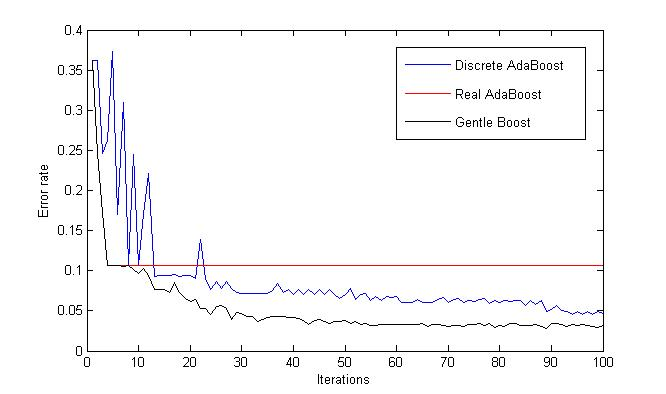
\includegraphics[width=0.7\textwidth]{loss_exp.jpg}
  	\caption{Error rates corresponding to \textsl{Discrete AdaBoost}, \textsl{Real AdaBoost} and \textsl{Gentle AdaBoost}.}
  	\label{loss_exp}
\end{figure}

\subsection{$L(y, F(\textbf{x})) = (y - F(\textbf{x}))^2$}

\subsection{$L(y, F(\textbf{x})) = \vert y - F(\textbf{x})\vert$}


\subsection{M-regression loss function}

\subsection{$L(y, F(\textbf{x})) = 2y^{*}F(\textbf{x}) - log(1+e^{2F(\textbf{x})})$}

\subsection{$L(y, F(\textbf{x})) = \log(1+e^{-2yF(\textbf{x})})$}

\section{Multi-class classification and some generalizations}

\subsection{A traditional approach}

\subsection{Some generalization of two-class algorithms}

\subsection{Other generalizations}

\section{Experiments}

\subsection{Experiments with simulated data}

\subsection{Experiments with real data}

\section{Conclusion}

\begin{thebibliography}{9999}%\enlargethispage{\baselineskip}
\bibitem[1]{boost}Friedman, J., Hastie, T. \& Tibshirani, R. \textsl{Additive Logistic Regression: a Statistical View of Boosting}, 2000.

\bibitem[2]{trebst}Friedman, J. \textsl{Greedy Function Approximation: A Gradient Boosting Machine}, IMS 1999 Reitz Lecture, 2001.

\bibitem[3]{SchaAndSin1998}Schapire, R.E. \& Singer, Y. \textsl{Improved Boosting Algorithms: Using Confidence-rated Predictions}, 1998.

\end{thebibliography}

\end{document}